\documentclass{article}
\usepackage{amsmath, amssymb, mathrsfs, xfrac, txfonts}
\usepackage{graphicx ,caption}
\usepackage[a4paper, total={7in,10in}]{geometry}
\usepackage{lmodern}
%\usepackage{hyperref}
\usepackage{array}
\def\arraystretch{2}
\newcolumntype{C}{>{$}c<{$}}
\newcolumntype{L}{>{$}l<{$}}
\newcolumntype{R}{>{$}r<{$}}
\DeclareSymbolFont{matha}{OML}{txmi}{m}{it}% txfonts
\DeclareMathSymbol{v}{\mathord}{matha}{118}
\begin{document}
\begin{titlepage}
\begin{center}
\textit{\today}
\vfill
\textbf{\LARGE{Condensé de la 1ère}\\\Large{Mathématiques}}\\
\vfill
\large{Ewen Le Bihan\\1eS3}
\end{center}
\end{titlepage}
\section*{Notations non vues en cours}
\begin{tabular}{c|l}
	$:=$ & Égal par définition\\
	$\mathbb{A} \cap \mathbb{B}$ & Appartient à la fois à $\mathbb{A}$ et à $\mathbb{B}$\\
	$\lceil x \rceil$ & Arrondir $x$ à l'entier supérieur. ($\lceil 5.1 \rceil = 6$)\\
	$1.5$ & Séparateur ,\\
	$x\cdot y$ & Multiplication $\times$\\
	$\vec{v} \:\bot\: \vec{u}$ & $\vec{v}$ et $\vec{u}$ orthogonaux
\end{tabular}
\pagestyle{empty}
\newpage
\tableofcontents
\pagestyle{empty}
\newpage


\pagestyle{plain}
\setcounter{page}{1}
\section{Polynômes du second degré $a x^2 + bx + c$}
\subsection{$\Delta$: Trouver les racines}
\begin{flalign*}
\Delta := b^2-4ac\\\\
\begin{cases}
	 \Delta > 0 & x_{1,2}=\frac{-b\pm \sqrt{\Delta}}{4a} \\
	 \Delta = 0 & x_0=\frac{b}{2a}\\
	 \Delta < 0 & \emptyset\\
\end{cases}
\end{flalign*}
\subsection{Étudier le signe}
Le signe du polynôme est celui de $a$, et, si $\Delta > 0$, est celui de $-a$ entre $x_1$ et $x_2$
\subsection{$\alpha$,$\beta$: Trouver l'extremum}
\subsubsection{Maximum ou minimum ?}
\begin{center}
\begin{tabular}{c|c}
	$a > 0$ & minimum\\
	$a < 0$ & maximum\\	
\end{tabular}
\end{center}
\subsubsection{Calcul}
\begin{flalign*}
\alpha &:= \frac{b}{2a}\\
\beta &:= \frac{\Delta}{4a}\\
\text{Sommet} &=(\alpha ; \beta)
\end{flalign*}
\begin{center}
Le polynôme atteint un extremum en $\alpha$ de valeur $\beta$
\end{center}
\subsection{Différentes formes}
\begin{center}
\begin{tabular}{c|l}
	Canonique & $(x-\alpha)^2+\beta$\\
	\hline
	Factorisée & $a(x-x_1)(x+x_2)$ \\ & $a(x_0-x)^2$\\
	\hline
	Développée & $a x^2 + bx +c$
\end{tabular}
\end{center}
\newpage


\section{Vecteurs $\vec{v}$, équations cartésiennes $ax+by+c=0$}
\subsection{Colinéarité} 
\begin{flalign*}
\vec{v} \:\&\: \vec{u} \text{ colinéaires} &\iff x_uy_v-y_ux_v=0 \\
&\iff (u) \parallel (v)\\
&\iff \vec{u} = \lambda \vec{v}\;\;\; (\forall \: \lambda \in \mathbb{R})
\end{flalign*}
\subsection{Vecteur directeur}
\subsubsection{Équation réduite $y = mx+p$}
\begin{flalign*}
\vec{v}\binom{1}{m}
\end{flalign*}
\subsubsection{Équation cartésienne $ax+by+c = 0$}
\begin{center}
\begin{tabular}{r|l}
Vecteur directeur & $\vec{v}\binom{-b}{a}$\\
Coefficient directeur & $m = -\frac{a}{b}$
\end{tabular}
\end{center}
\subsection{Décomposer un vecteur}
\begin{flalign*}
(\forall \: \lambda, \lambda' \in \mathbb{R}) \;\;\; \vec{w} = \lambda \vec{v} + \lambda' \vec{u}\\
\end{flalign*}
% TODO finish this section
\subsection{Relation de Chasles}
\begin{flalign*}
\overrightarrow{AC} = \overrightarrow{AB} + \overrightarrow{BC}
\end{flalign*}
\newpage


\section{Statistiques}
\subsection{Caractéristiques}
\begin{center}
\begin{tabular}{c|c|rl}
	Nom & Type & Formule\\
	\hline
	Effectif total & /& $N:=$ & $\sum_{i=0}^{p}n_i$\\
	Moyenne & Centrale & $\bar{x}:=$ &  $ \frac{1}{N}\sum_{i=0}^{p}n_ix_i$ \\
	Médiane & Centrale & $Me:=$ & 
$\begin{cases}$
$N \text{ pair}\;\;\; &\frac{1}{2}\left( x_{\frac{N}{2}} + x_{\frac{N+1}{2}}\right)\\$
$N \text{ impair}\;\;\;&x_{\left\lceil\frac{N}{2}\right\rceil}$
$\end{cases}$\\
	Mode & Centrale & $Mo:=$ &Valeur ou classe qui a l'effectif le plus grand\\
	Premier Quartil & Non-centrale & $Q_1:=$ & $ x_{\left\lceil\frac{N}{4}\right\rceil}$\\
	Troisième Quartil & Non-centrale & $Q_3:=$ & $ x_{\left\lceil\frac{3}{4}N\right\rceil}$\\
	Étendue & Dispersion & $e:=$ & $ x_{max} - x_{min}$\\
	Écart inter-quartil & Dispersion & & $Q_3 - Q_1$\\
	Variance & Dispersion & $V :=$ & $\frac{1}{N}\sum_{i=0}^{p}(n_ix_i^2) - \bar{x}$\\
	Écart type & Dispersion & $\sigma :=$ & $\sqrt{V}$
\end{tabular}
\end{center}
\subsection{Transformation de valeurs selon $y=mx+p$}
\begin{flalign*}
\bar{y} &= m\bar{x}+p\\
V_y&=m^2V_x\\
\sigma_y &= |m|\sigma_x
\end{flalign*}
\newpage


\section{Probabilités}
\subsection{Notions}
\begin{center}
\begin{tabular}{c|c|l}
Nom & Symbole & Description\\\hline
Univers & $\Omega$ & Ensemble des issues possibles\\
Variable aléatoire & $X$ & Fonction qui renvoie un nombre aléatoire dans $\Omega$\\
\end{tabular}
\end{center}
\subsection{Loi de probabilité de $X$}
Exemple: 
\begin{itemize}
	\item $\Omega = \{0;1;2\}$
	\item $p(X=0)=p(X=2)=\frac{1}{4}$
	\item $p(X=1)=\frac{1}{2}$
\end{itemize}
\begin{center}
\begin{tabular}{r||c|c|c}
k & \;\;0\;\; & \;\;1\;\; & \;\;2\;\;\\
\hline
$p(X=k)$ & $\frac{1}{4}$ & $\frac{1}{2}$ & $\frac{1}{4}$
\end{tabular}
\end{center}
\subsection{Caractéristiques}
\begin{center}
\begin{tabular}{c|l|rl}
	Nom & Description & Formule\\
	\hline
	Espérance & Résultat moyen espéré & $E(X) :=$ & $\sum_{i=1}^{n}p_ix_i$\\
	Variance & & $V(X) :=$ & $\sum_{i=1}^{n}(p_ix_i) - E(X)^2$\\
	Écart type && $\sigma(X) :=$ & $\sqrt{V(X)}$
\end{tabular}
\end{center}
\subsection{Issues, évennements}
Exemple:\\
\begin{tabular}{r||c|c}
	$x_i$ & A & B\\
	\hline
	$p(X=x_i)$ & $\frac{1}{3}$ & $\frac{2}{3}$\\
\end{tabular}
\\\\\\
Calcul de l'issue $AB$ ($A \to B$):
\begin{flalign*}
p(AB) &= p(A)\cdot p(B)
\end{flalign*}
Calcul de l'évenement $\Theta$ << au moins une fois $A$ >>:
\begin{flalign*}
p(\Theta) &= p(AB) + p(BA) + p(AA)
\end{flalign*}
Calcul de l'évennement contraire $\bar{\Theta}$:
\begin{flalign*}
p(\bar{\Theta}) = 1 - p(\Theta)
\end{flalign*}


\newpage
\subsection{Loi binomiale $\mathscr{B}$}
\subsubsection{Définitions}
\begin{center}
\begin{tabular}{r|l}
	Épreuve de Bernoulli \\
	\hline
	Évenement << succès >> & $S$\\
	Évenement << échec >> & $\bar{S}$\\
	Probabilité de succès & $p := p(S)$\\
	Probabilité d'échec & $q := p(\bar{S})$\\&\;\;\;\;$= 1 - p$\\\\
	Schéma de Bernouilli & $\mathscr{B}(n;p)$\\\hline
	Nombre de répétitions & $n$\\
	Nombre de succès & $k$\\
	Univers & $\Omega = [0;n]\cap \mathbb{N}$
	
\end{tabular}
\end{center}
\subsubsection{Loi de $X$}
Si $X \sim \mathscr{B}(n;p)$
\begin{center}
\begin{tabular}{c||c|c|c|c|c}
	$k$ & 0 & 2 & 3 & ... & $n$\\\hline
	$p(X=k)$ & $\binom{n}{k}p^kq^{n-k}$
\end{tabular}
\end{center}
\subsubsection{Caractéristiques}
$$\forall k \in [0;n] \cap \mathbb{N}$$
\begin{flalign*}
E(X)&=np\\
V(X)&=npq
\end{flalign*}
\newpage

\section{Suites $U_n$}
\subsection{Types de suites}
\subsubsection{Fonctionnelle}
$$U_n=2n$$
\subsubsection{Récursive}
\begin{flalign*}
	\begin{cases}
    	U_{n+1}&=U_0+U_n\\
    	U_0&=5
	\end{cases}
\end{flalign*}
\subsection{Suites remarquables}
\subsubsection{Arithmétiques}
$$
\begin{cases}
U_{n+1}&=U_n + r\\
U_0&=k\\
\end{cases}
$$$$
U_n=U_0+r\cdot n
$$
\subsubsection{Géométriques}
$$
\begin{cases}
U_{n+1}&=U_n\cdot q\\
U_0 &= k
\end{cases}
$$$$
U_n=U_0\cdot q^n
$$
\subsection{Sommes}
\subsubsection{Suites arithmétiques}
\begin{flalign*}
	\sum_{\mu=i}^{j}U_\mu=\frac{U_i+U_j}{2} \cdot (j-i+1)
\end{flalign*}
\subsubsection{Suites géométriques}
\begin{flalign*}
	\sum_{\mu=i}^{j}U_\mu=U_i\cdot \frac{1-q^{j-i+1}}{1-q}
\end{flalign*}
\subsection{Variations}
\subsubsection{Fonction associée}
\begin{flalign*}
(\forall n \in \mathbb{N}) & f:n\mapsto U_n
\\
\text{Si } f \nearrow/\searrow &\implies U_n \nearrow/\searrow
\end{flalign*}
\subsubsection{Méthode 2}
$$U_{n+1}-U_n\lessgtr0\iff U_n \searrow / \nearrow$$
\subsubsection{Méthode 3}
$$\frac{U_{n+1}}{U_n}\lesseqgtr 1 \iff U_n \nearrow / \searrow$$

\newpage
\section{Produit Scalaire $\vec{u} \cdot \vec{v}$}
Note: pour éviter les confusions, la multiplication normale est notée $\times$ dans ce chapitre.
\subsection{Calcul}
\begin{center}
$\vec{\mu}, \vec{\kappa}$  projetés orthogonaux de $\vec{u}$ et $\vec{v}$
\end{center}
\begin{flalign*}
    	\vec{u} \cdot \vec{v} &\iff ||\vec{u}|| \times ||\vec{v}|| \times \cos{(\vec{u};\vec{v})}\\
    	&\iff x_u\times x_v+y_u\times y_{v}\;\text{*}\\
		&\iff \vec{u} \:\bot\: \vec{v}\\
		&\iff \vec{\mu} \cdot \vec{\kappa}\\
		&\iff \frac{1}{2} \left(||\vec{u}||^2 + ||\vec{v}||^2 - ||\vec{v}-\vec{u}||^2\right) \text{**}
\end{flalign*}
*  Seulement dans un repère orthonormé\\
** Si $\vec{u}$ et $\vec{v}$ sont vecteurs directeurs des segments formant un triangle:
\begin{figure}[htp]
\centering
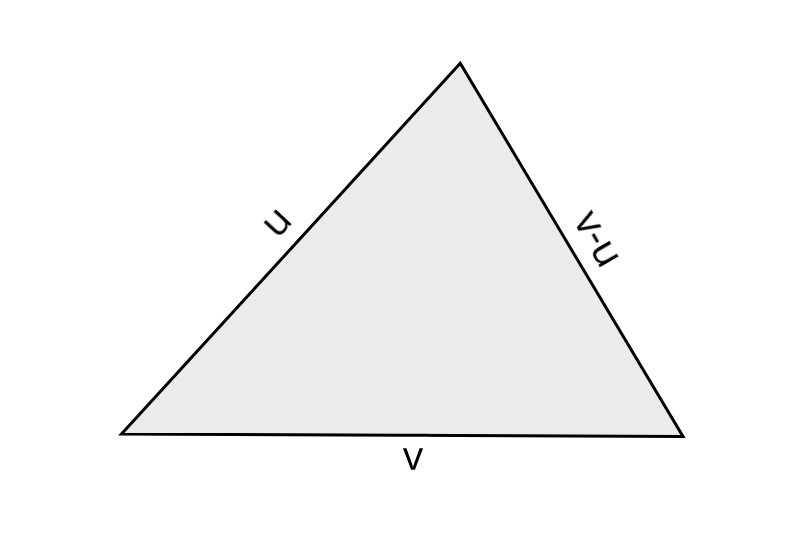
\includegraphics[scale=0.25]{prodscal_triangle_1}
\caption{}
\label{}
\end{figure}

\subsection{Multiplication de segments liés}
Si $A, H, B$ alignés dans cet ordre
\begin{flalign*}
\overrightarrow{AB} \cdot \overrightarrow{AC} = AB \times AH
\end{flalign*}
Sinon, si $H, A, B$ alignés dans cet ordre
\begin{flalign*}
\overrightarrow{AB} \cdot \overrightarrow{AC} = -AB \times AH
\end{flalign*}
\subsection{Identités remarquables}
\begin{flalign*}
||\vec{u} \pm \vec{v}||^2 &= ||\vec{u}||^2 \pm 2 \vec{v}  \cdot \vec{u} + ||\vec{v}||^2\\
(\vec{u}-\vec{v})(\vec{u}+\vec{v}) &=||\vec{u}||^2 - ||\vec{v}||^2
\end{flalign*}
\subsection{Angle aigu et obtu}
\setlength{\belowdisplayskip}{0pt}
$$\vec{u} \cdot \vec{v} > 0 \iff (\vec{u}; \vec{v}) \text{ aigu}\\$$
\begin{center}
	Et inversement
\end{center}

\newpage
\section{Étude de fonctions}
\subsection{Fonctions de bases}
\begin{center}
\begin{tabular}{C|CCC}
	x & -\infty & 0 & +\infty \\\hline
	x & \nearrow & 0 & \nearrow\\
	x^2 & \searrow & 0 & \nearrow\\
	\sfrac{1}{x} & \searrow & || & \searrow\\
	\sqrt{x} & ///// & 0 & \nearrow\\
	|x| & \searrow & 0 & \nearrow
	
\end{tabular}
\end{center}

\subsection{Opérations sur fonctions}
$\leftrightarrows$ : Changement de variation\\
$\rightrightarrows$ : Même variation
\begin{center}
$\forall \: k \in \mathbb{R}$,\;
$\forall \: \lambda_+ \in \mathbb{R}^+$,\;
$\forall \: \lambda_- \in \mathbb{R}^- $\\

\begin{tabular}{C|CCC}
	u & -\infty & 0 & +\infty\\\hline
	u + k & \rightrightarrows & k & \rightrightarrows\\
	u \cdot \lambda_+ & \rightrightarrows & 0 & \rightrightarrows\\
	u \cdot \lambda_- & \leftrightarrows & 0 & \leftrightarrows\\
	\sqrt{u} & ///// & 0 & \nearrow\\
	\sfrac{1}{u} & \searrow & || & \searrow\\
\end{tabular}
\end{center}

\newpage
\subsection{Dérivées}
\subsubsection{Nombre dérivé $f'(a)$}
\begin{flalign*}
f'(a) = \lim_{h\to0} \frac{f(a+h) - f(a)}{h}
\end{flalign*}
\subsubsection{Tangeante $T$ au point $a$}
\begin{flalign*}
T:y=\underbrace{f'(a)}_{\text{coef dir}}(x-a)+f(a)
\end{flalign*}
\subsubsection{Dérivées remarquables}
\begin{center}

$\forall \: n \in \mathbb{N} \;\;\; $
\begin{tabular}{C|C}
	f(x) & f'(x)\\\hline
	\text{constante} & 0\\
	x^n & nx^{n-1}\\
	\sqrt{x} & 1/2 \sqrt{x}\\
	\sfrac{1}{x} & - 1/x^2\\
\end{tabular}
\end{center}
\subsubsection{Opérations sur les dérivées}
\begin{center}
$(u+v)'$ et $(ku)'$ fonctionne normalement.
\begin{flalign*}
(uv)' &= u'v+v'u\\
\left(\frac{u}{v}\right)' &= -\:\frac{v'u-u'v}{v^2}\\
%\left(\frac{1}{v}\right)' & -\frac{v'}{v^2}\\
\end{flalign*}
\end{center}
\subsubsection{Utilisations de $f'(x)$}
Sens de variation de $f$\\
\begin{center}
%TODO truc sur les tableaux de signes. Genre mx+p: -oo: sgn(-a), +oo: sgn(a)
Si $f$ dérivable sur $[I;J]$\\
\begin{tabular}{C|CC}
	x & I  & J \\\hline
	f'(x) & + & -\\\hline
	f(x) & \nearrow & \searrow
\end{tabular}
\end{center}
Extrema (\textit{et pas <<extremums>> bordel de merde})\\
\begin{flalign*}
\text{Trouver le(s) $x$ pour } f'(x) = 0
\end{flalign*}

\section{Trigonométrie}
\subsection{Notions}
\begin{description}	
	\item[Radians] Mesure d'angle $\in [0;2\pi]$ (principalement)\\
	\item[Cercle trigonométrique] cercle de rayon 1 ($2\pi r \to 2\pi$)
\end{description}
\subsection{Valeurs remarquables}
\begin{figure}[htp]
\centering
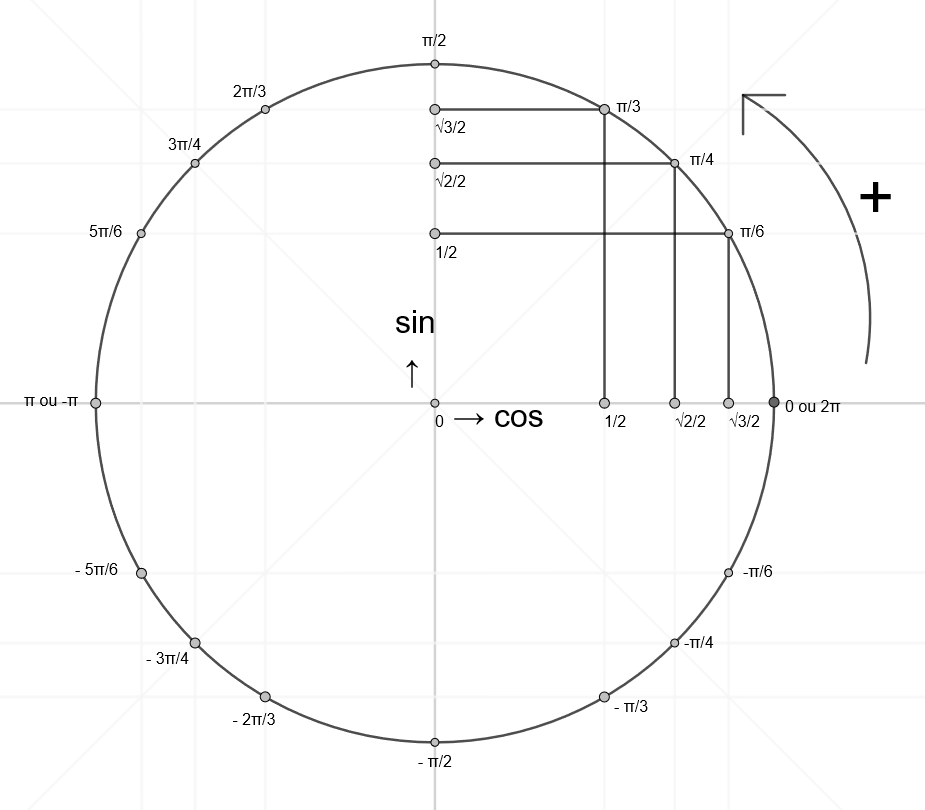
\includegraphics[scale=0.25]{cercle-trigo-filled}
\caption{}
\label{}
\end{figure}

\subsection{Formules de trigonométrie}

\begin{equation*}
\end{equation*}


\end{document}
